\documentclass{report}
\usepackage{graphicx}
\usepackage{titlesec}
\usepackage{wrapfig}
\usepackage{placeins}

\title{Lab 1: Battery Evaluation}
\date{September 9th, 2022}
\author{Brady Moore \\
    Nataly Panczyk}

\begin{document}
\maketitle
\section{Statement of Purpose}
In ECE 205 lecture, we deal with ideal voltage and current sources, but in real life, there are no such things.
In this lab, we will use a battery, which is a device which converts chemical energy into electrical energy.
Even though we typically think of batteries as ideal voltage sources, we will characterize ways in which the battery differs from the ideal voltage source.

\section{Procedure}
The first step in this lab is to measure the open circuit voltage ($V_{OC}$) for each of the three batteries tested in this experiment.
We did this by connecting a multimeter in parallel with each battery and recording the displayed voltage once it stabilized as shown in Fig.~\ref{fig:SchemA}. Then, we modified
the circuit by adding a 100 $\Omega$ resistor connected in series with the battery. For each battery, we connected the multimeter in parallel
across the resistor and recorded the voltage once it stabilized as shown in Fig.~\ref{fig:SchemB}.


The next step in this lab was to calculate the current flowing in each circuit (which changed according to the battery tested). Using Equation \ref{ohms_law}
(Ohm's Law), we can calculate the current using our measured voltage across the resistor ($V_r$) and the resistance of the resistor ($R$).
Then, we can use the calculated current values for each battery ($I_1$, $I_2$, $I_3$) to calculate the internal resistance of the battery using
the previously measured open circuit voltage ($V_{OC}$). We do this again, using Ohm's Law, rewritten as $V_{OC} = IR_{int}$, where $R_{int}$
is the internal resistance of the resistor. We repeat this calculation with the values shown in Table \ref{tab:results}.

    \begin{equation}
        \label{ohms_law}
        V = IR
    \end{equation}
\begin{figure}[htpb]
    \centering
    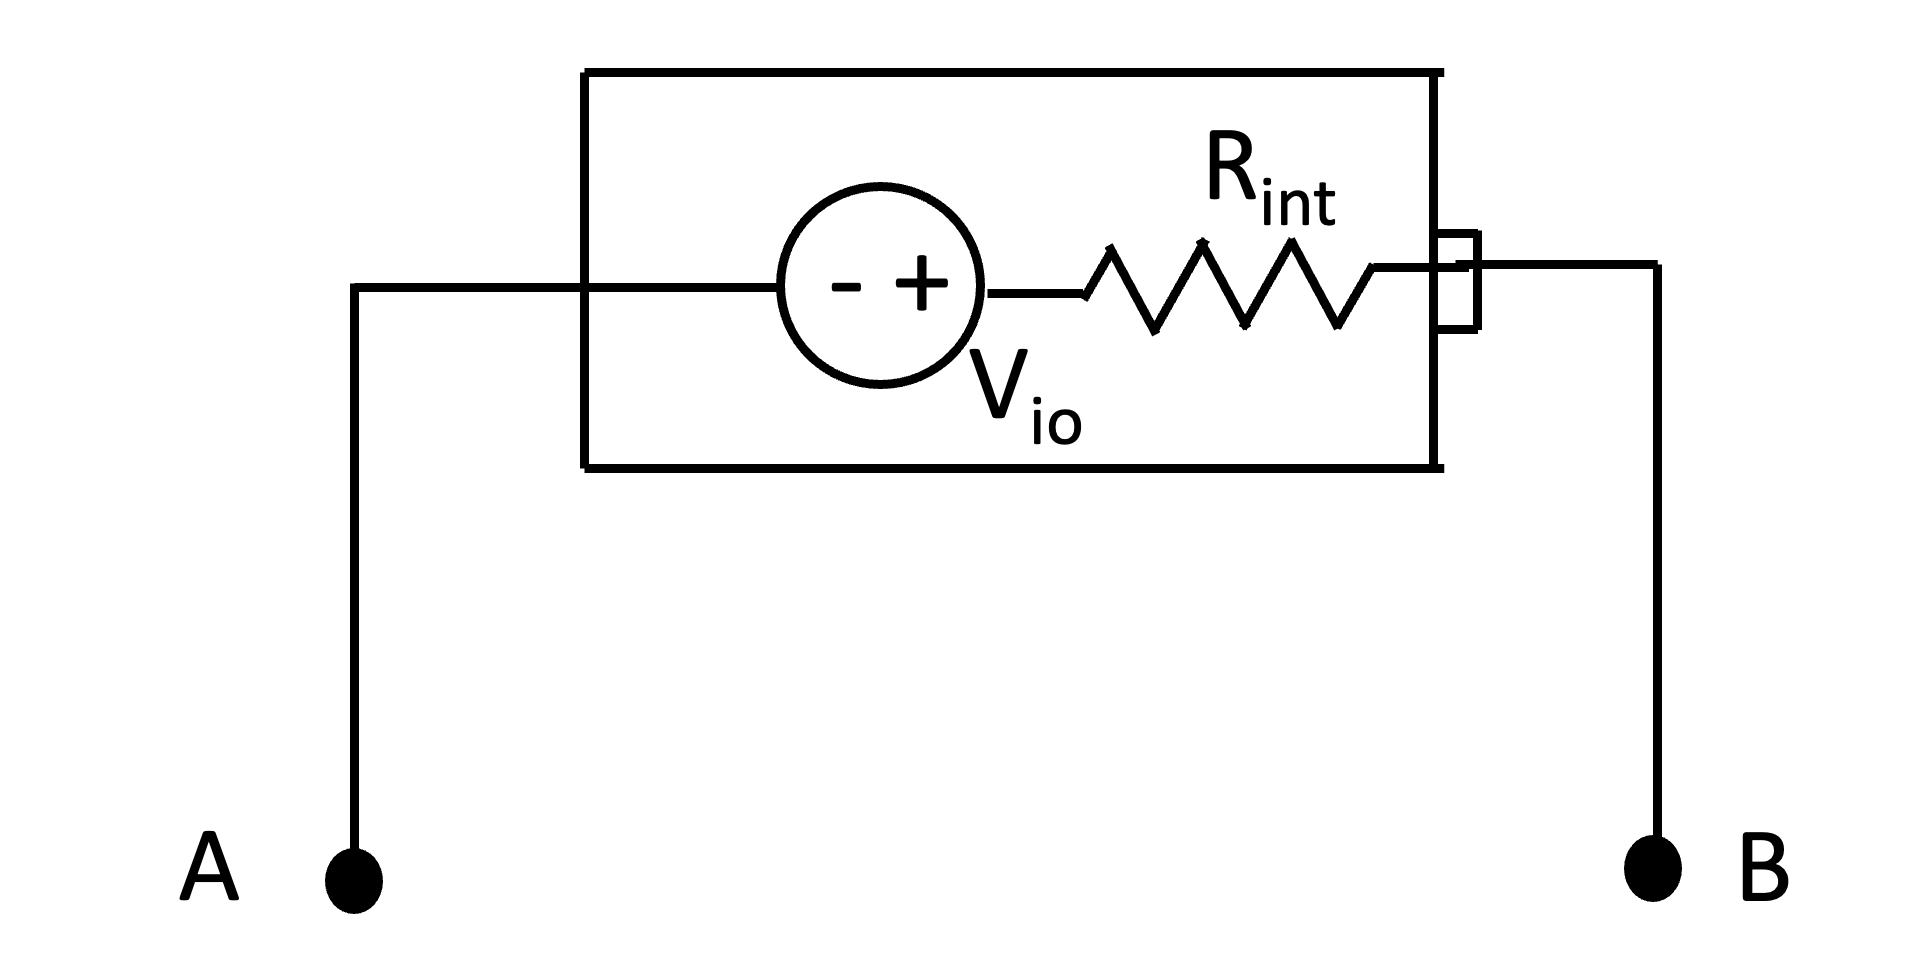
\includegraphics[width=0.8\textwidth]{SchematicA.png}
    \caption{A schematic showing how $V_{oc}$ was measured.}
    \label{fig:SchemA}
\end{figure}
\begin{figure}[htpb]
    \centering
    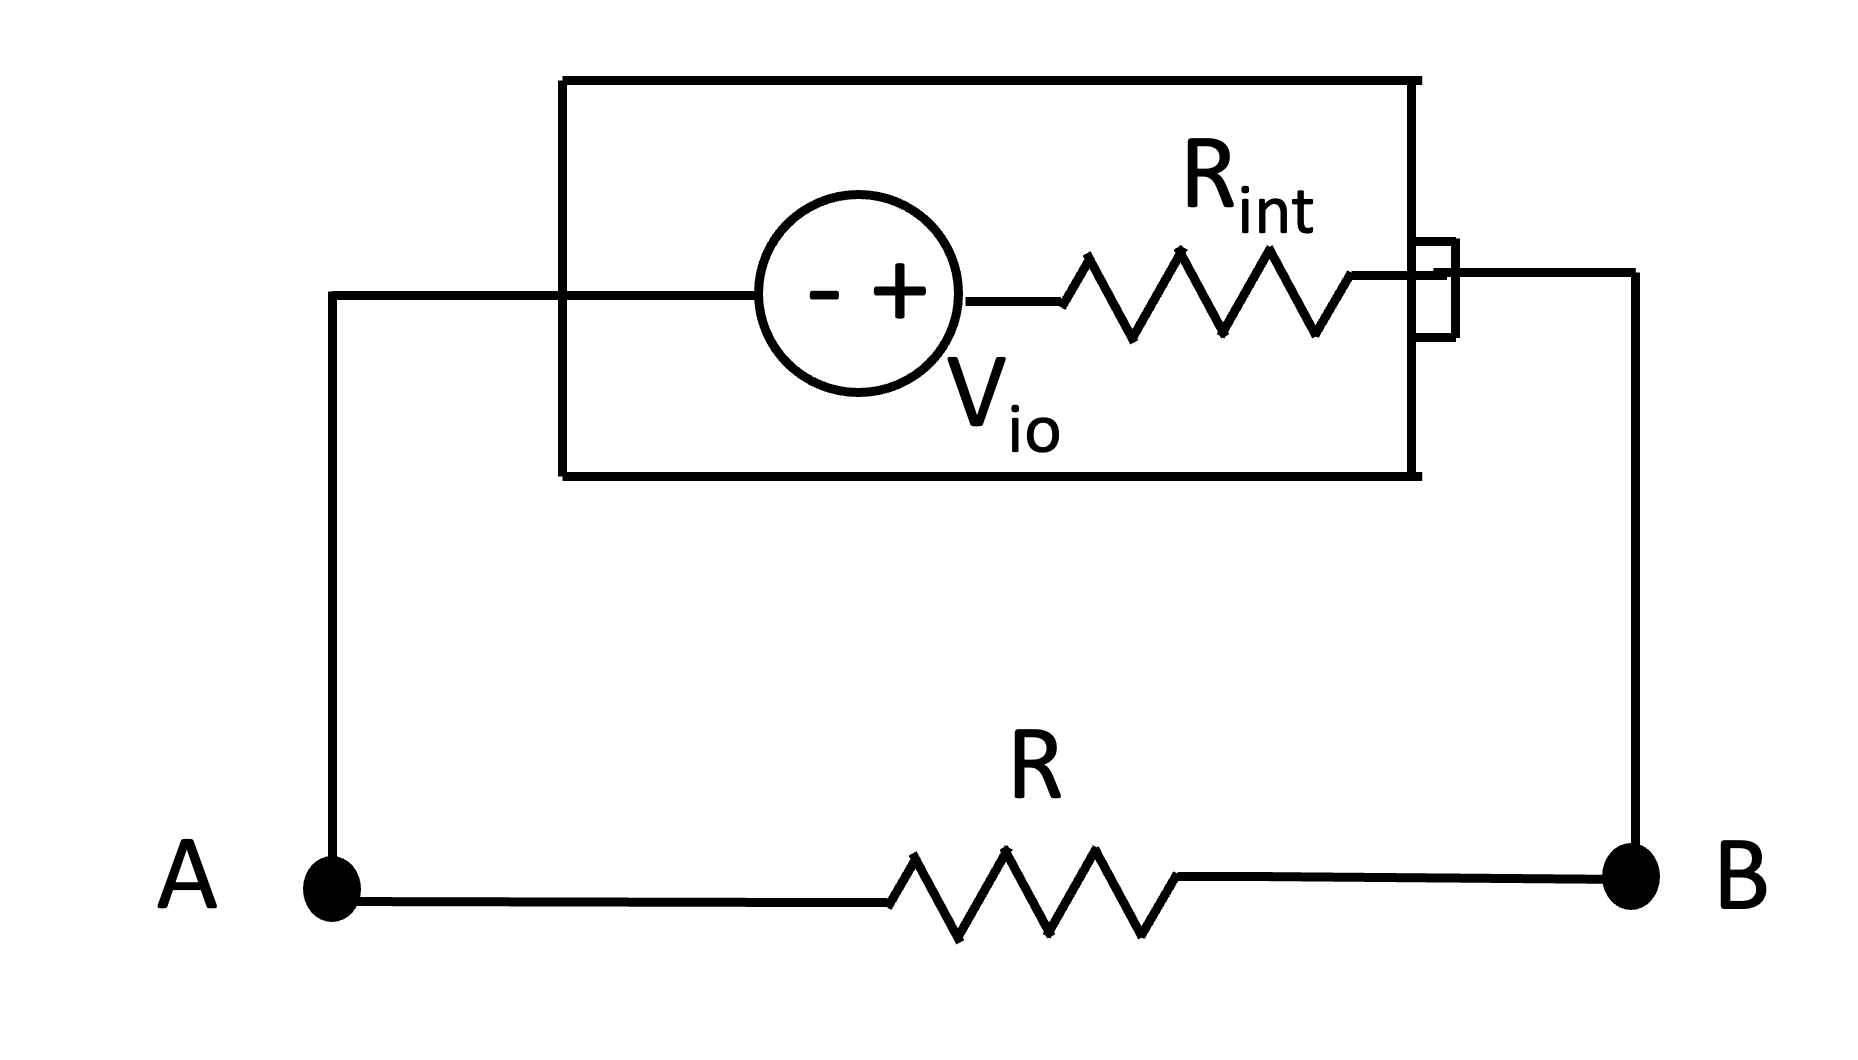
\includegraphics[width=0.8\textwidth]{SchematicB.png}
    \caption{A schematic showing how $V_{ab}$ was measured.}
    \label{fig:SchemB}
\end{figure}
\section{Raw Data}
\FloatBarrier
\begin{table}[h!]
    \centering
    \caption{Experimental values of $V_{oc}$ and $V_{ab}$ for all three batteries. The current and $R_{int}$ columns are calculated using Eq.~\ref{}}
    \label{tab:results}
    \begin{tabular}{|c c c c c|}
        \hline
        Battery & $V_{oc} [V]$ & $V_{ab} [V]$ & $ I[A]$ & $R_{int} [\Omega]$\\
        \hline
        A      &   1.6044    &  1.5918     &  0.015918     &  0.79155 \\
        B   & 1.6072    & 1.6025 &  0.016025 & 0.2933 \\
        C   & 1.6083    & 1.5865    & 0.015865  & 1.3741 \\
        \hline

    \end{tabular}
    \end{table}
    \FloatBarrier
\section{Analysis}
The voltage meausered across the battery is the open load voltage, $V_{oc}$,because there is no load or current flowing.
$V_{ab}$ is the voltage drop across the 100 $\Omega$ resistor.
$V_{ab}$ can be used to find the current flowing through the circuit according to Ohm's Law Eq.~\ref{ohms_law}.
The current in addition to $V_{oc}$ can be used to calculate the internal resistance according to the following equation:
\begin{equation}
    V_{oc} = I(R+R_{int})
\end{equation}
where $R$ is the resistance of the added resistor.
For this lab $R = 100 \Omega$.
\begin{equation}
    R_{int} = \frac{V_{oc}}{I}-R
\end{equation}
The calculated $R_{int}$ values are tabulated in Table~\ref{tab:results}.

The diffence in internal resistance can be due to a variety of factors including the temperature, brand of battery, and how depleted the battery is.
In this lab, our internal resistances were on the order of 1 $\Omega$.

\section{Results and Conclusion}
This experiment demonstrated a method to calculate the internal resistance of a battery that accumulates over time with its use.
To accomplish this, we measured the open circuit voltage, the voltage across the resistor connected in series with the battery, and utilized Ohm's Law to calculate the internal resistance of each battery.
Complications with this experiment included the fluctuating nature of the voltage readings on the multimeter, which never fully stabilized and could contribute to errors in our final calculations.
One application of this experiment is that the results could be used to evaluate the performance of different brands of batteries over their lifetimes by measuring the accumulated internal resistance.
Overall, we observed very few challenges in producing quality results for this experiment.
\end{document}
